%%%%%%%%%%%%%%%%%%%%%%%%%%%%%%%%%%%%%%%%%%%%%%%%%%%%%%%%%%%%%%%%
%%%%%%%%%%%%%%%%%%%%%%%%%%% Metadata %%%%%%%%%%%%%%%%%%%%%%%%%%%
%%%%%%%%%%%%%%%%%%%%%%%%%%%%%%%%%%%%%%%%%%%%%%%%%%%%%%%%%%%%%%%%
\documentclass{Axon}

\title{Is Reality as We Experience It Real and Does it Make Life Worthwhile?}

\authors{
    \addauthor{Albert Einstein}{einstein@minkowsi.com}
    \addauthor{Paul Erdös}{erdos@stimulant.edu}
    \addauthor{Alan Turing}{turing@bombe.gov}
}

\addbibresource{Bibliography.bib}
%%%%%%%%%%%%%%%%%%%%%%%%%%%%%%%%%%%%%%%%%%%%%%%%%%%%%%%%%%%%%%%%
%%%%%%%%%%%%%%%%%%%%%%%%%%%%% Paper %%%%%%%%%%%%%%%%%%%%%%%%%%%%
%%%%%%%%%%%%%%%%%%%%%%%%%%%%%%%%%%%%%%%%%%%%%%%%%%%%%%%%%%%%%%%%
\begin{document}
\maketitle
\makeauthor
%%%%%%%%%%%%%%%%%%%%%%%%%%%%%%%%%%%%%%%%%%%%%%%%%%%%%%%%%%%%%%%%
%%%%%%%%%%%%%%%%%%%%%%%%%%% Abstract %%%%%%%%%%%%%%%%%%%%%%%%%%%
%%%%%%%%%%%%%%%%%%%%%%%%%%%%%%%%%%%%%%%%%%%%%%%%%%%%%%%%%%%%%%%%
\begin{abstract}
In this groundbreaking, highly speculative, and very serious paper, we tackle two of the most profound questions ever pondered by humankind: “Why do things exist?” and “Does existence matter?” Leveraging the combined intellects of Einstein’s relativity, Turing’s computational theories, and Erdös’ prolific caffeinated collaborations, we propose that existence is not merely a cosmic happenstance but a necessity driven by the universal laws of physics, mathematics, and late-night coffee-fueled epiphanies.

Our findings suggest that the universe exists because it can, much like an overachieving graduate student with too many research grants. Existence is the ultimate flex of potentiality, a sandbox where particles, energy, and ideas collide in a spectacular display of cosmic creativity. Furthermore, the mattering of existence is a subjective endeavor, bestowed with meaning by self-aware entities who have too much free time on their hands.
\end{abstract}
%%%%%%%%%%%%%%%%%%%%%%%%%%%%%%%%%%%%%%%%%%%%%%%%%%%%%%%%%%%%%%%%
%%%%%%%%%%%%%%%%%%%%%%%%%%% Section 1 %%%%%%%%%%%%%%%%%%%%%%%%%%
%%%%%%%%%%%%%%%%%%%%%%%%%%%%%%%%%%%%%%%%%%%%%%%%%%%%%%%%%%%%%%%%
\section{Why do things exist?}
Alright, let's tackle the big one: "Why do things exist?" Look, the universe is a pretty wild place. We're talking about 13.8 billion years of cosmic chaos, exploding stars, and random quantum fluctuations. So why does stuff exist? Because it can, and because it had to. It's the ultimate flex of possibility.

\begin{example}
    Imagine if the universe were a cooking show. You’ve got a dash of gravity, a sprinkle of strong nuclear force, and just a pinch of electromagnetism. Mix that all together, and what do you get? The cosmos – a cosmic souffle that, against all odds, didn’t collapse in on itself (most of the time). Existence isn’t just a happy accident; it’s the ultimate recipe cooked up by the laws of physics. So, why do things exist? Because, somewhere in the multiverse, a Gordon Ramsay of creation screamed, "It’s RAW!" and the universe had no choice but to get itself together.
\end{example}

Imagine a blank canvas with infinite potential. Now, throw some paint on it. That's the Big Bang. Suddenly, you've got particles, energy, forces – all the ingredients for making stuff. The universe is like a cosmic sandbox where the laws of physics play out in real-time, creating stars, planets, and eventually, us. It’s not that things exist for some grand purpose; they exist because, statistically, they’re bound to show up when you have enough time and space.

Think about it: out of nothing, you get everything. It's like rolling dice with an infinite number of sides. Sooner or later, you're going to get every possible outcome. We’re one of those outcomes. So, why do things exist? Because existence is the path of least resistance. It’s the default state when you have a universe full of potential and a few billion years to spare.

\begin{itemize}
    \item Why does this paper exist?
    \item The answer lies herein.
    \item The End
\end{itemize}

In the end, existence is just a byproduct of the universe being the universe. It’s not personal; it’s physics. The real magic isn't in why things exist but in the fact that they do, and we get to ponder it. So, why not kick back and enjoy the ride?
%%%%%%%%%%%%%%%%%%%%%%%%%%%%%%%%%%%%%%%%%%%%%%%%%%%%%%%%%%%%%%%%
%%%%%%%%%%%%%%%%%%%%%%%%%%% Section 2 %%%%%%%%%%%%%%%%%%%%%%%%%%
%%%%%%%%%%%%%%%%%%%%%%%%%%%%%%%%%%%%%%%%%%%%%%%%%%%%%%%%%%%%%%%%
\section{Does existence matter?}
Well, let's cut through the cosmic fluff and hit the core. It matters if you want it to \cite{MALAJETMAROVA2017209}. Existence is like an open-source project. It’s there, running in the background, but its value is entirely up to the contributors – us.

From the universe's perspective, existence is just a sequence of events, particles bouncing around, energy shifting. It’s indifferent, like a machine running its code. But here’s the kicker: we’re part of the code. We’re self-aware subroutines capable of asking if it all matters. That’s pretty wild if you think about it.

\begin{equation}
    \boldsymbol{\sigma} = \frac{1}{J} \left(\frac{K}{2}(J^2-1)\boldsymbol{I}+\mu J^{-\frac{2}{3}} dev(\mathbf{F} \cdot \mathbf{F}^\intercal)\right) \in \mathbb{R}
\end{equation}

So, does it matter? Depends on your frame of reference. On a cosmic scale, probably not. Stars explode, galaxies collide, and the universe keeps trucking along. But on a human scale, hell yeah, it matters. It matters because we make it matter. We assign meaning to our experiences, relationships, and pursuits \cite{quantumTomfoolery2024}. We create art, solve problems, and ask big questions. In the grand scheme, it's our ability to give a damn that gives existence its punch.

Ultimately, existence matters because we decide it does. It’s like playing a video game – the pixels on the screen don’t care, but the player sure does. We’re the players in this grand, indifferent game. So, if you want existence to matter, make it matter. It's your call.
%%%%%%%%%%%%%%%%%%%%%%%%%%%%%%%%%%%%%%%%%%%%%%%%%%%%%%%%%%%%%%%%
%%%%%%%%%%%%%%%%%%%%%%%%%%% Section 3 %%%%%%%%%%%%%%%%%%%%%%%%%%
%%%%%%%%%%%%%%%%%%%%%%%%%%%%%%%%%%%%%%%%%%%%%%%%%%%%%%%%%%%%%%%%
\section{An Attempt at a Conclusion}
Alright, let's wrap this \textcolor{red}{cosmic} \textcolor{purple}{mind} \textcolor{blue}{trip up}. Why do things exist? Because the universe is a giant sandbox with infinite potential, and stuff just happens \cite{quantumJokes}. It’s physics doing its thing. And does existence matter? Only if you want it to. The universe doesn’t care, but we do, and that’s what gives life its kick.

\begin{figure}[h]
    \centering
    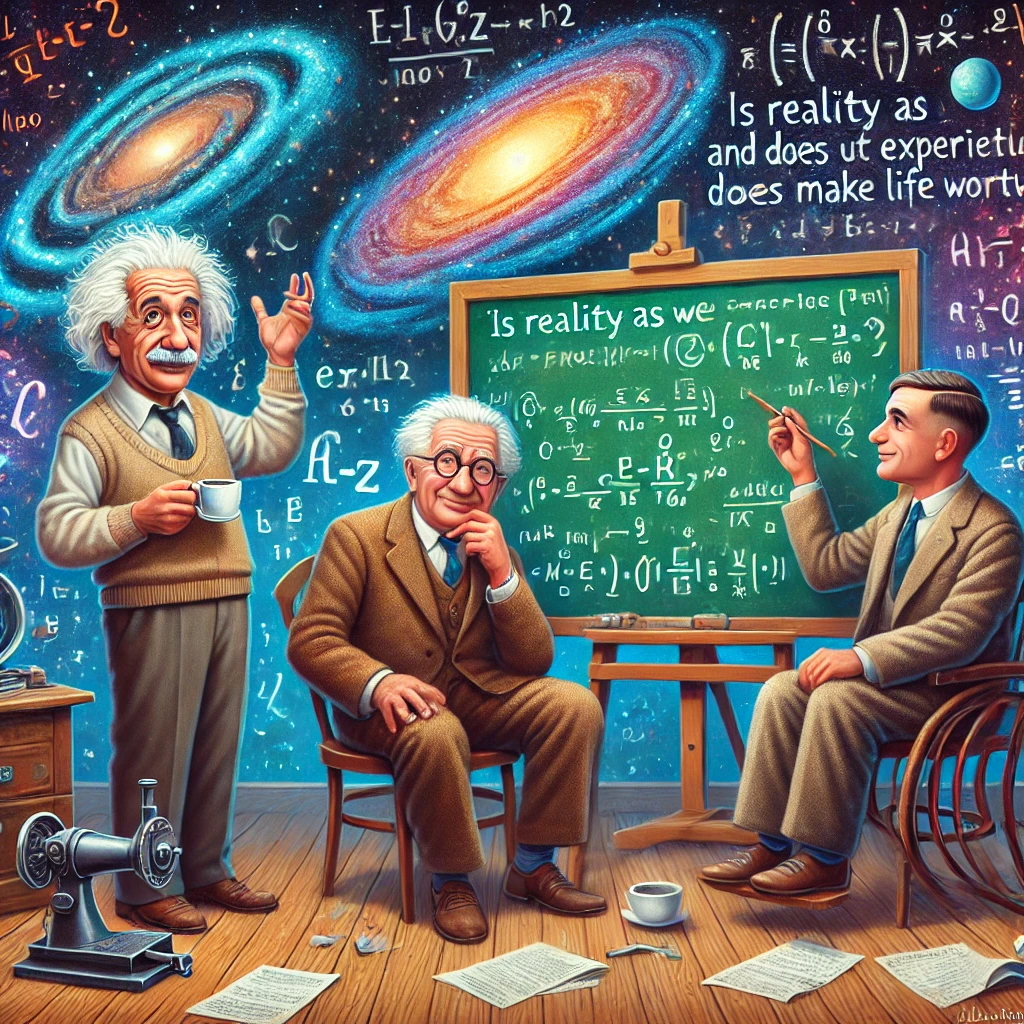
\includegraphics[width=0.35\linewidth]{TheGang.jpeg}
    \caption{The Gang Pondering | Circa 2092}
    \label{fig:The Gang}
\end{figure}

In the end, existence is both everything and nothing. It’s the ultimate paradox, a cosmic joke with us as the punchline. So, what’s the takeaway? Embrace the chaos, find your own meaning, and remember: the universe is indifferent, but you don't have to be. Welcome to the ride.

\printbibliography

\end{document}